\documentclass{article}
% Packages
\usepackage{amsmath} % For mathematical symbols and equations
\usepackage{graphicx} % For including images
\usepackage{cite} % For managing citations
\usepackage{lipsum} % For generating dummy text
\usepackage{algorithm} % For writing algorithms
\usepackage{algpseudocode} % For writing pseudocode
\usepackage[a4paper, total={6in, 8in}]{geometry}

\pagenumbering{arabic} % Arabic/Indic page numbers

\begin{document}
\begin{titlepage}
    \begin{center}
        \vspace*{1cm}

        \Large
        \textbf{Vehicle Cruise Control System: Modeling, Simulation, and Control Analysis in Matlab/Simulink}

       \vspace{0.5cm}
        Cyber-Physical Systems Report 
            
        \vspace{1.5cm}
        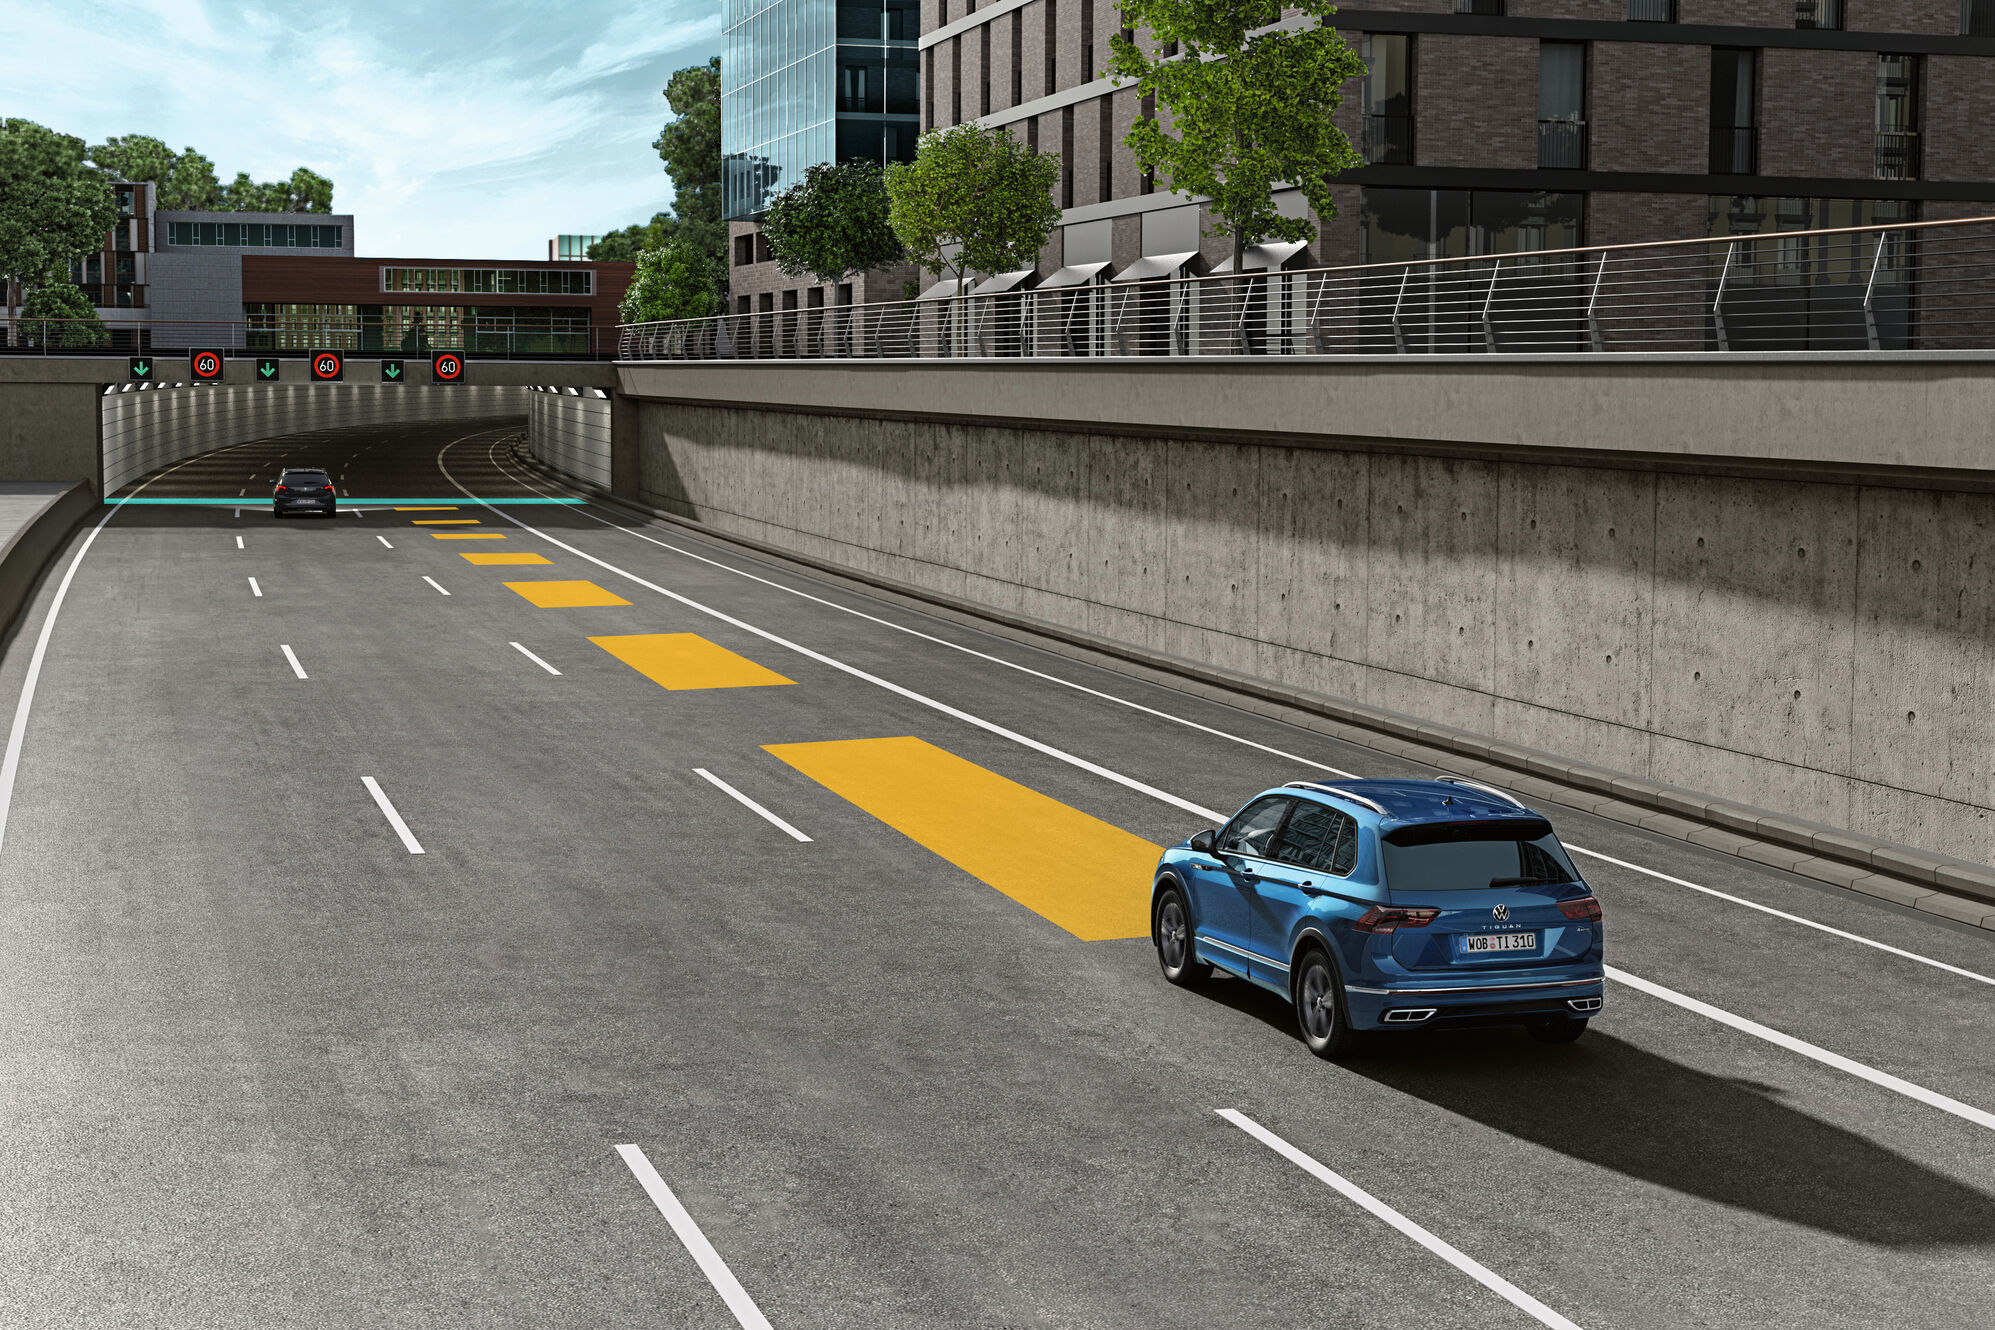
\includegraphics[width=1\textwidth]{img/cc.jpeg}

       \vfill

        \textbf{Abhishta Gatya Adyatma}
            
        \vspace{0.8cm}
                 
        Faculty of Information Technology\\
        Brno University of Technology\\
        26 April 2024
            
   \end{center}
\end{titlepage}

\tableofcontents
\newpage

\section{Introduction}

Cyber-physical systems (CPS) integrate computational algorithms with physical components, enabling digital control over physical interactions. This interdisciplinary field empowers engineers, scientists, and researchers to model, simulate, and control complex systems via digital communications. Handling such complications, a power tool called MATLAB developed by MathWorks, serves as the cornerstone for designing, simulating, and implementing CPS. Its versatile toolboxes facilitate the modeling of dynamic systems, data analysis, and algorithm deployment to embedded platforms.

CPS finds applications across diverse industries including automotive, robotics, infrastructure, and architecture. In this context, the author explores a specific CPS application: Vehicle Cruise Control. This feature automates vehicle speed control, particularly beneficial for long drives on straight roads like interstates. By analyzing this system using MATLAB, the author aims to experiment with different parameters and control strategies, providing insights into CPS implementation and optimization.

\section{Theoretical Foundations}

\begin{figure}[H]
    \centering
    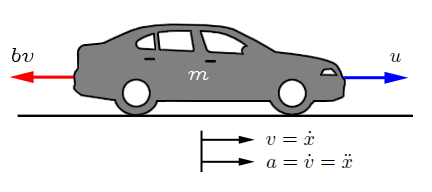
\includegraphics[width=0.7\linewidth]{img/cruise_control_schematic.png}
    \caption{Simplified Vehicle Cruise Control Model (ctms.engin.umich.edu/CTMS/index.php)}
    \label{fig:enter-label}
\end{figure}

Vehicle Cruise Control is a feedback-based control system designed to maintain a constant speed for the vehicle despite external disturbances. It continuously monitors the vehicle's speed output and compares it to a desired reference speed. This comparison enables automatic adjustments to the throttle input. In this project, the author simplifies the vehicle's dynamics focusing on the vehicle's mass and damping coefficient.

\begin{table}[H]
    \centering
    \begin{tabular}{ccc}
         Variable & Description & Unit \\
         \hline
         m & Mass & kg \\ 
         b & Damping Coefficient & N * s / m \\
    \end{tabular}
    \caption{Simplified Vehicle Cruise Control Model System Parameters}
    \label{tab:units}
\end{table}

Table \ref{tab:units} shows the model's system parameters, where the vehicle's mass is expressed in Kilograms (kg) and the Damping Coefficients are expressed in Newton seconds per meter. The Damping Coefficient quantifies the damping force acting against the vehicle's motion. It represents the resistance encountered by the vehicle due to factors such as rolling resistance and aerodynamic drag. With only these parameters, the system is simplified to a mass-damper system in the first order by summing up the forces in the x-direction, further expressed in Equation \ref{eq:de}.

\begin{equation}
    m\dot{v}+bv=x
    \label{eq:de}
\end{equation}

The differential equation represents the forces acting on the vehicle, including inertia and damping, in response to the control force applied to the vehicle. The Laplace transformation of the equation converts it from the time domain to the Laplace domain, providing a mathematical tool for analyzing the system's behavior and response to inputs more conveniently. The Laplace-transformed equation is expressed as shown in Equation \ref{eq:tf}, where $V(s)$ represents the velocity of the vehicle in the Laplace domain and $U(s)$ represents the control force input in the Laplace domain. This transfer function describes the relationship between the Laplace-transformed velocity and control force input.

\begin{equation}
\frac{V(s)}{U(s)} = \frac{1}{ms + b}
\label{eq:tf}
\end{equation}

This transfer function provides insights into how the vehicle's velocity responds to changes in the control force input, considering the inertia and damping effects of the vehicle dynamics. However, this system is not complete without a feedback control mechanism that would reliably and effectively regulate the vehicle's speed throughout varied conditions. A Proportional-Integral-Derivative (PID) Controller, chosen by the author, calculates the output control signal based on three components \cite{pid:2020}:

\begin{itemize}
    \item Proportional (P): produces an output proportional to the error signal. It provides immediate corrective action in proportion to the current error.
    \item Integral (I):  produces an output proportional to the accumulated (integral) error signal. This allows the controller to eliminate steady-state error between the setpoint and system output.
    \item Derivative (D): provides a control signal proportional to the time rate of change of the error signal. It permits a faster system transient response without increasing the percent overshoot.
\end{itemize}

In summary, the PID controller calculates the system output with corrective actions to minimize steady-state error and achieve a fast transient response. Formally defined in Equation \ref{eq:pid} where $u(t)$ is the output control signal, $e(t)$ is the error signal, $K_p$, $K_i$, and $K_d$ are the proportional, integral, and derivative gain constant. Equation \ref{eq:pidl} shows PID in the Laplace Domain.

\begin{equation}
    u(t) = K_p e(t) + K_i \int_0^t e(\tau) d\tau + K_d \frac{de(t)}{dt}
    \label{eq:pid}
\end{equation}

\begin{equation}
    U(s) = K_p E(s) + K_i \frac{E(s)}{s} + K_d s E(s)
    \label{eq:pidl}
\end{equation}

With the control system in place, the cruise control system can be analyzed in its transient response, studying how the system responds to changes in the control input and how it settles into a new steady-state condition (the desired output). Key aspects to analyze from the transient response are the Rise Time (time taken to reach 90\% of the desired value), Settling Time (time taken for the system to settle to the desired value), Peak Time (time taken for the system to reach the maximum value), Overshoot and Undershoot (the maximum value the system exceeds or falls below before settling), and the Steady State Error (difference between the desired steady-state value and the actual steady-state value of the system).

\section{Modeling, Simulation, Control, and Result}

\begin{figure}[H]
    \centering
    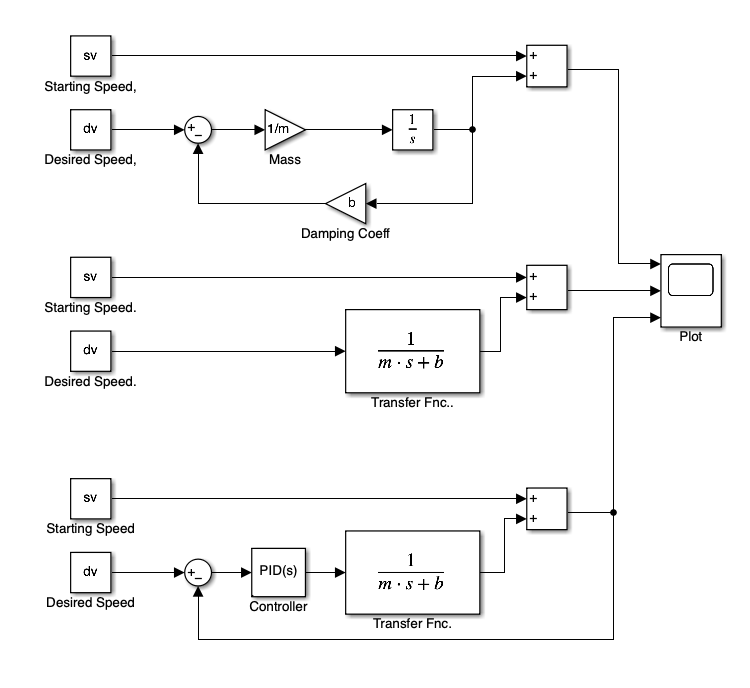
\includegraphics[width=0.8\linewidth]{img/block_diagram.png}
    \caption{Block Diagram of the Vehicle Cruise Control System (with/without feedback control)}
    \label{fig:block}
\end{figure}

The model of the Vehicle Cruise Control System in Matlab/Simulink is depicted in Figure \ref{fig:block}. The top section represents the system's dynamics using a Differential Equation. The middle section illustrates the system's behavior through a Transfer Function in the Laplace Domain. Finally, the bottom section demonstrates the implementation of a feedback control system using a PID Controller. As previously discussed, the transfer function characterizes the relationship between the vehicle's speed (output) and the control force (input). By incorporating the PID Controller, the system can dynamically adjust the control force to regulate the vehicle's speed, gradually aligning it with the desired speed set by the cruise control system. Further, the author will discuss the results of simulation and experimentation using the above model.

\subsection{Stability of the System}

Before simulating the system, it's essential to note that the Transfer Function of the model is stable. Stability is critical in the Vehicle Cruise Control System because the system needs to converge to a stable point across various parameters to match the desired speed from the current speed. To assess the system's stability, the author conducted a Pole-Zero Map analysis \cite{pzmap:2005}. This evaluation confirms whether the system, with the specified parameters, lies within stable regions, ensuring its reliability and effectiveness in regulating vehicle speed.

\begin{figure}[htbp]
    \centering
    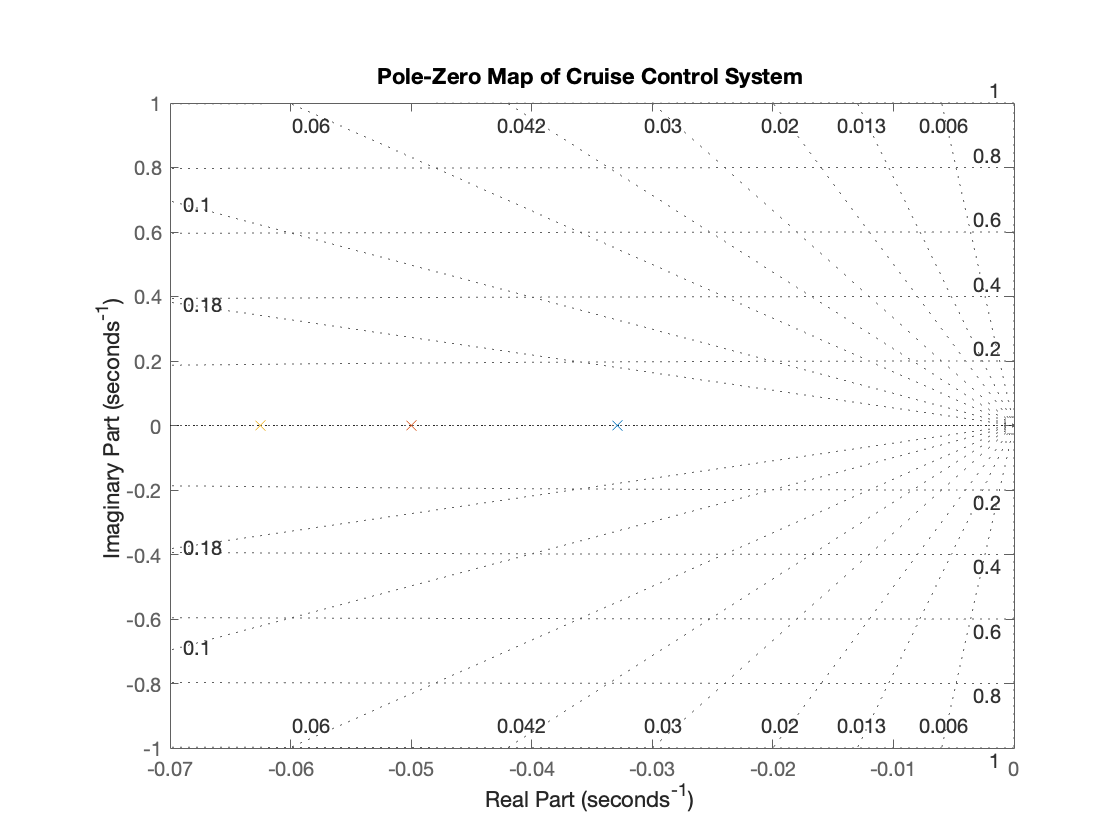
\includegraphics[width=0.7\linewidth]{img/pzmap_cc.png}
    \caption{Pole-Zero Map of Vehicle Cruise Control with 3 Distinct Configuration}
    \label{fig:pzmap}
\end{figure}

Figure \ref{fig:pzmap} displays the Pole-Zero Map of the Vehicle Cruise Control System with 3 Distinct Configuration ($m=760 kg;b=25 N*m/s$; $m=1000 kg;b=50 N*m/s$; $m=1200 kg;b=75 N*m/s$). The figure shows that all three configurations lie within the stable regions of the map. This enables the author to use this Transfer Function as a Vehicle Cruise Control System knowing its stability throughout different linearly incrementing configurations.

\subsection{Simulation and Control}

During the simulation and control of the model, the author utilized three different cars, each with varying masses, as configurations for the experiment. This facilitated the examination of the speed responses of different vehicles to the implemented cruise control system.

\begin{table}[H]
    \centering
    \begin{tabular}{c|c}
        Vehicle & Mass \\
        \hline
        Wuling Air EV & 888 kg \\
        Mitsubishi Xpander & 1,220 kg \\
        Volkswagen Tiguan & 1,703 kg \\
    \end{tabular}
    \caption{Configuration of Vehicles Mass (Approximation)}
    \label{tab:mass}
\end{table}

\subsubsection{Transient Response Analysis of Variability in Damping Coefficient}

The damping coefficient of a vehicle varies depending on its conditions and specifications. For demonstration purposes, the author will apply the same damping coefficient to all specified vehicles listed in Table \ref{tab:mass} and explore various values. This experiment aims to showcase the performance of the Vehicle Cruise Control System and identify the optimal damping coefficient corresponding to each vehicle's mass specification.

\begin{figure}[htbp]
    \centering
    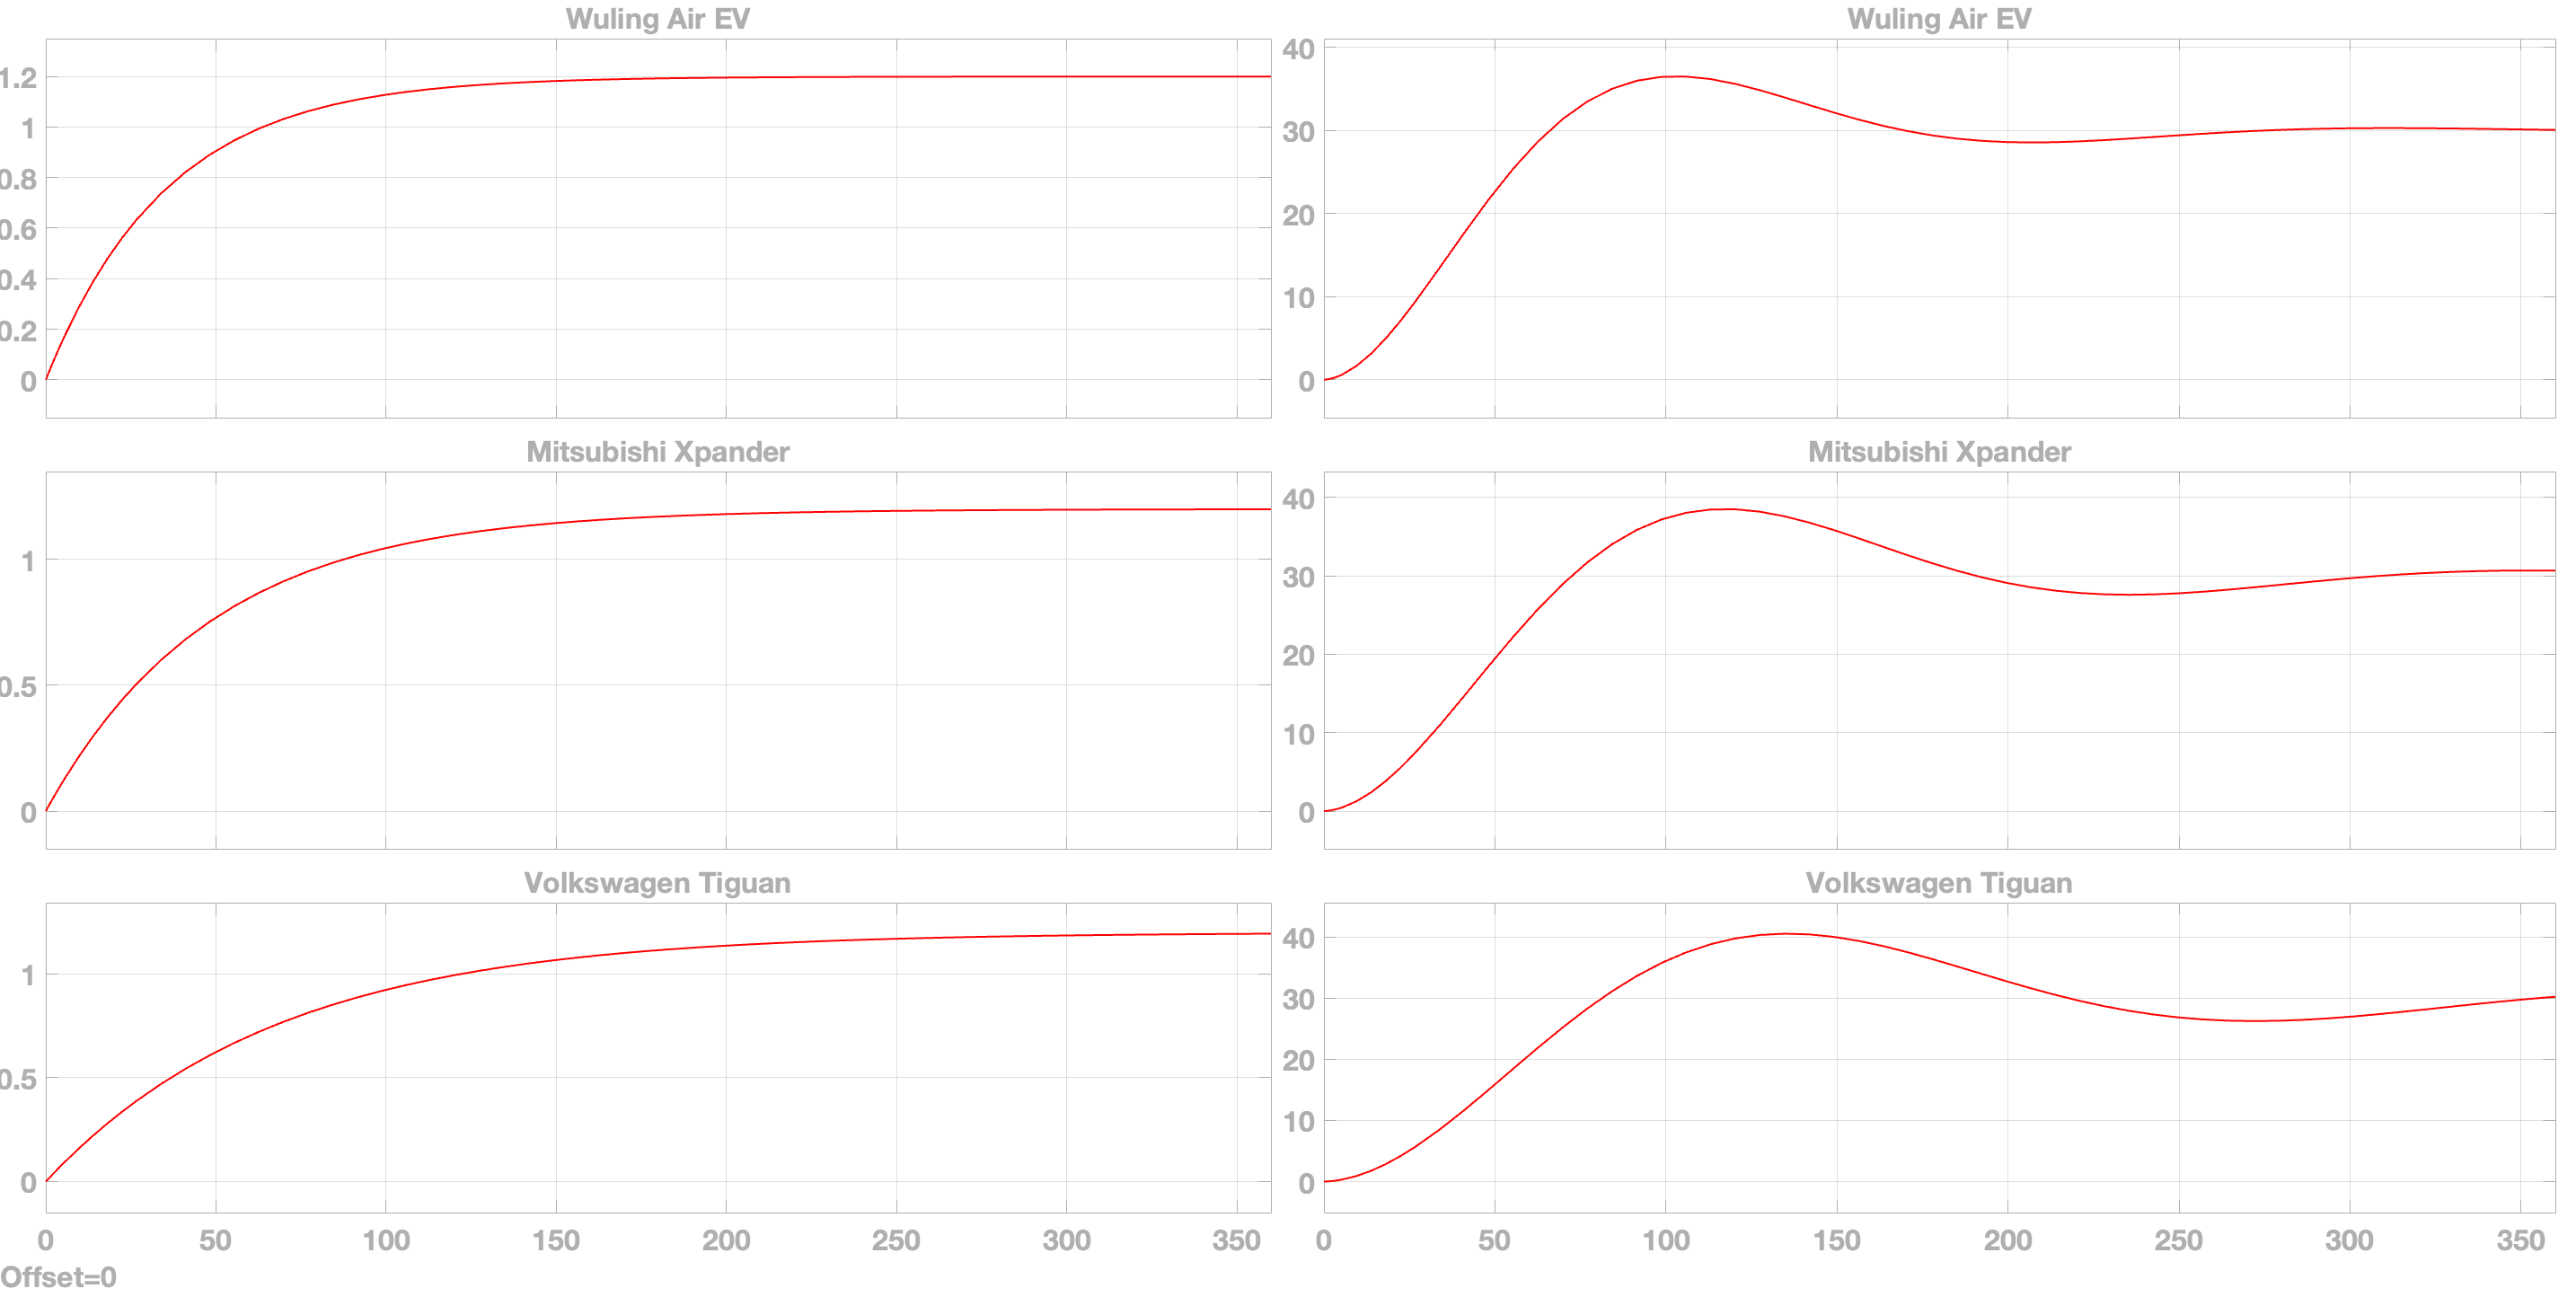
\includegraphics[width=1\linewidth]{img/25_Nms.png}
    \caption{Vehicles Cruise Control System Responses (25 N*m/s)}
    \label{fig:25nms}
\end{figure}

Starting from $0 m/s$ to a desired output of $30 m/s$ and using a damping coefficient of $25 N*m / s$, Figure \ref{fig:25nms} illustrates the system's response to the input signal with and without a PID Controller. The response shows that this configuration has an overshoot of $~5 m/s$ in velocity, an undershoot of $~2 m/s$, a peak time of $100 - 120$ seconds, and a settling time of $200 - 300$ seconds. Comparing the vehicle's response to the system reveals that the Wuling Air EV (888 kg) achieves faster settling time and minimal overshoot compared to the heavier Mitsubishi Xpander (1,220 kg) and Volkswagen Tiguan (1,703 kg). Furthermore, as vehicle mass increases, both overshoot and undershoot grow, alongside the rise time. Hence, heavier vehicles like the Mitsubishi Xpander and Volkswagen Tiguan require a larger damping coefficient to attain a faster settling time, as deduced from the analysis.

\begin{figure}[htbp]
    \centering
    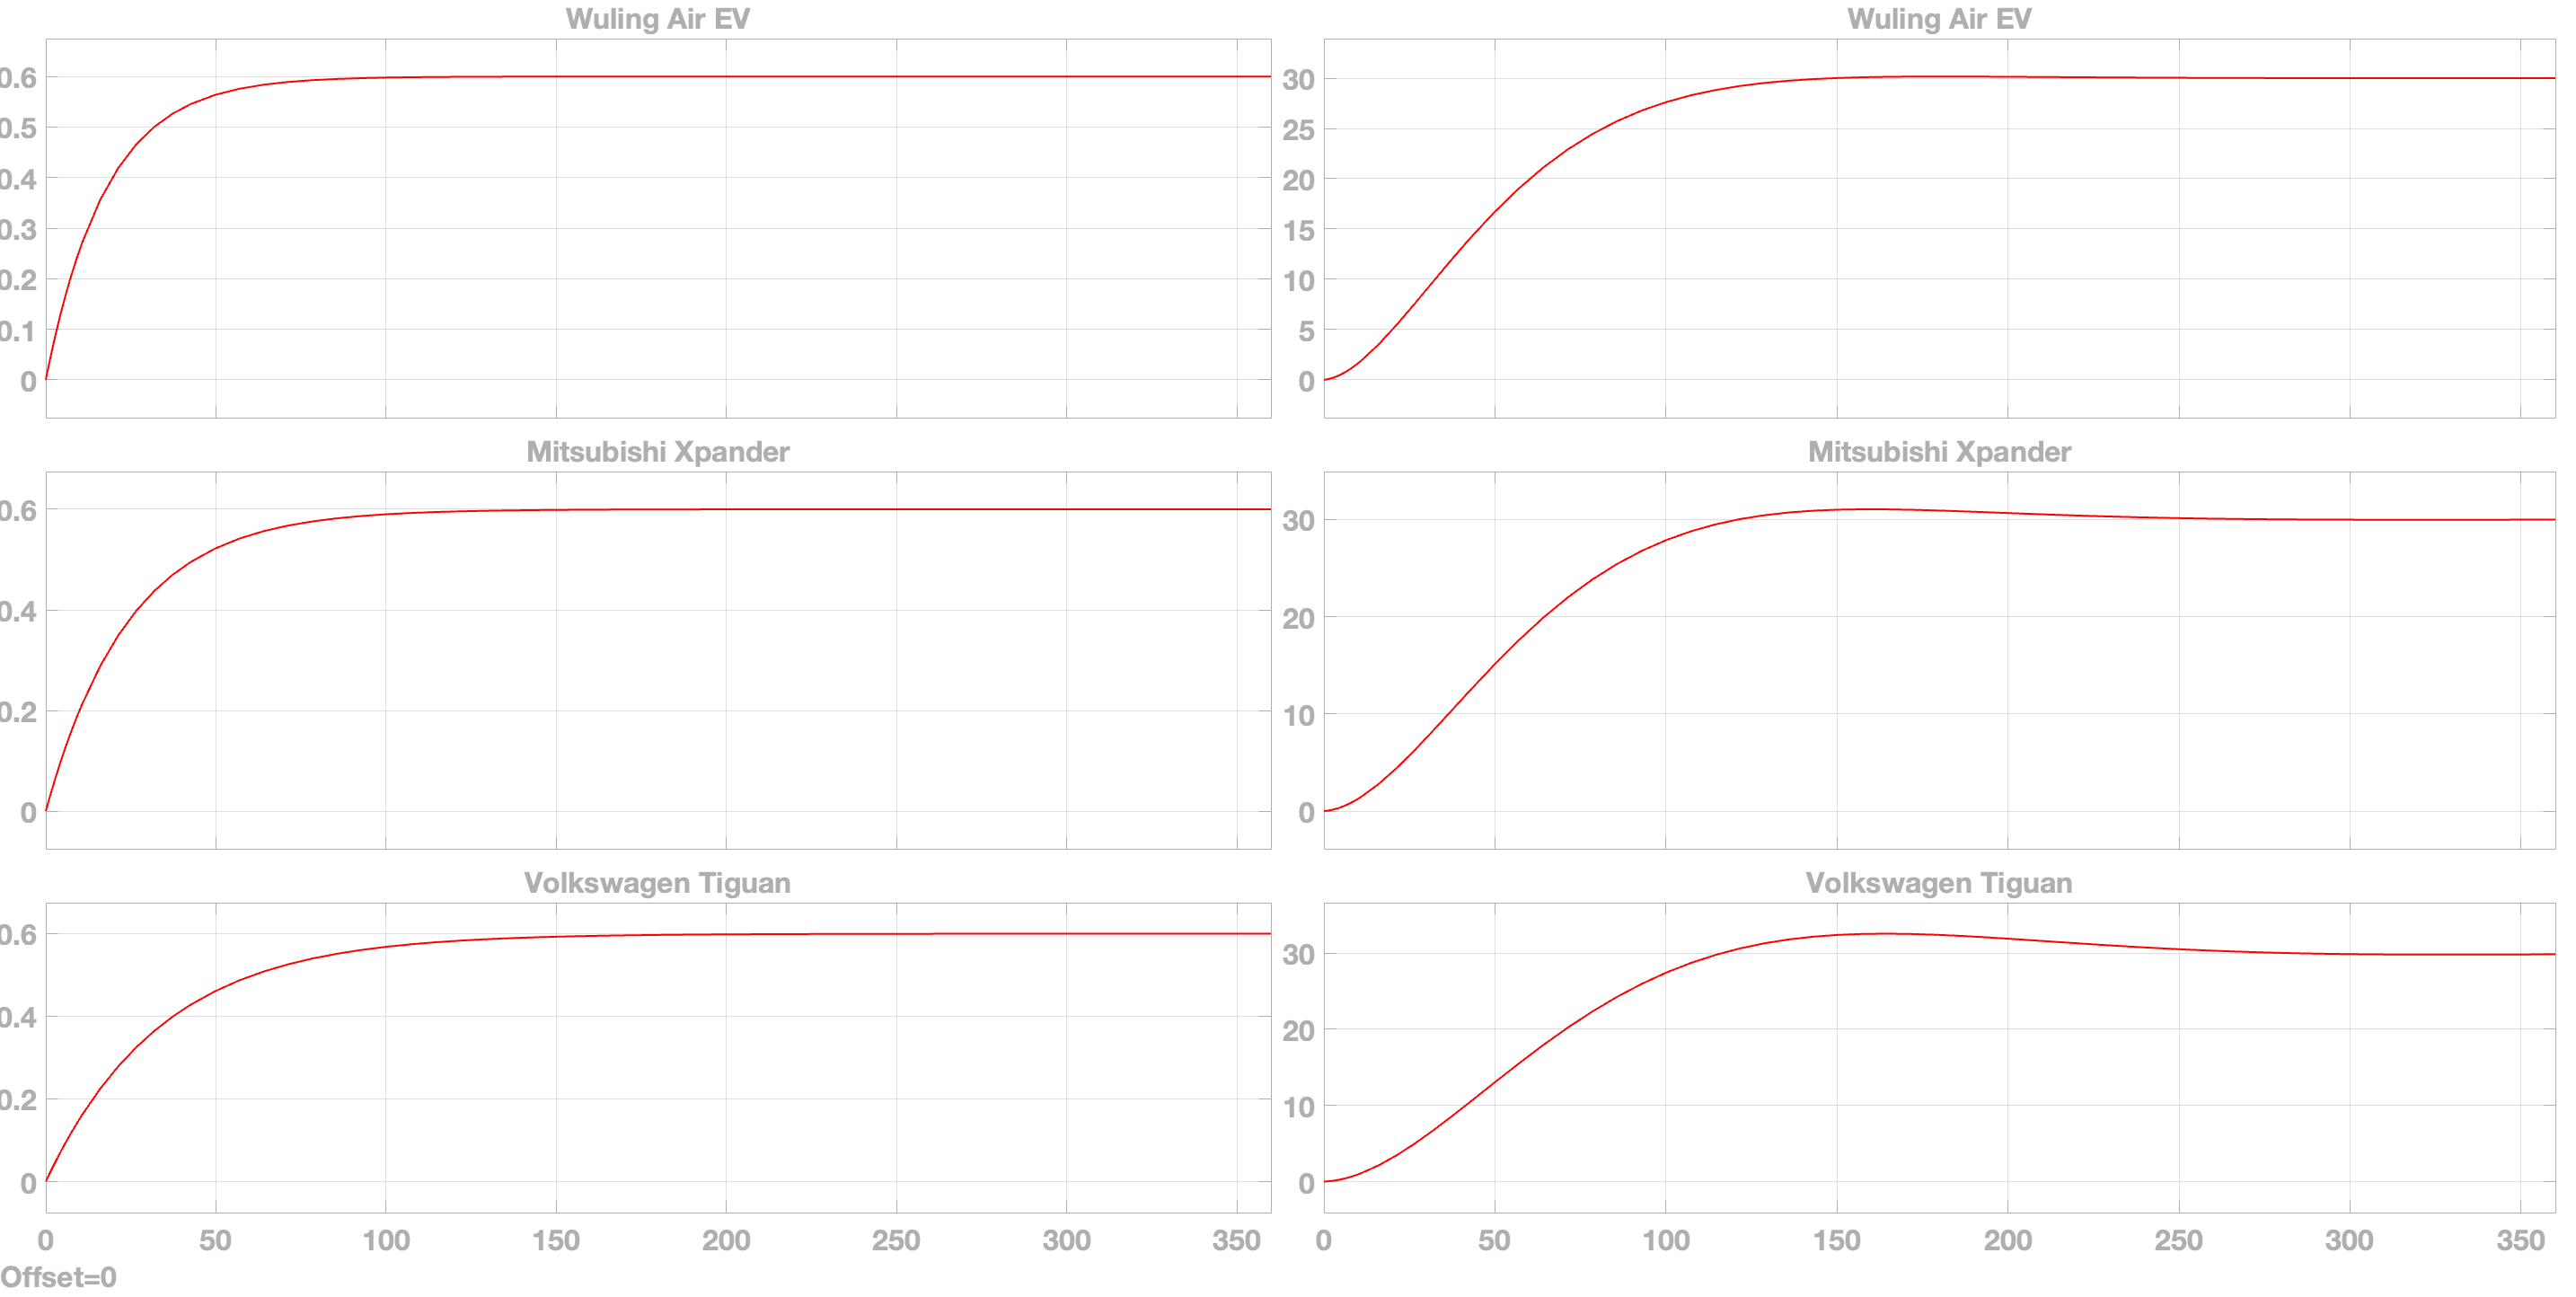
\includegraphics[width=1\linewidth]{img/50_Nms.png}
    \caption{Vehicles Cruise Control System Responses (50 N*m/s)}
    \label{fig:50nms}
\end{figure}

Using $50 m/s$ it is clear that the system produces less overshoot and undershoot to reach a steady state. Having an overshoot of $0 - 2 m/s$, a peak time of approximately $150$ seconds, followed by a settling time close to its peak time. However, using a higher damping coefficient prolongs the rise time, peak time, and settling time of the system since more resistive force is applied. This might not be ideal for some cases where the vehicle needs to achieve a faster settling time but with a reasonable overshoot. Further, the author experiments with the parameters of the Proportion, Integral, and Derivative of the PID Control to optimize the system. 

\subsubsection{Transient Response Analysis of Variability in PID Controller Parameters}

To recap the PID Controller, the Proportional Gain immediately adjusts the output in proportion to the current error, the Integral Gain eliminates steady-state error between the setpoint and system output, and the Derivative Gain enhances the system's transient response without amplifying overshoot. Adjusting the gains of each component enables the system to more effectively converge toward the desired output. With this, the author experimented on each component to analyze the transient response.

\begin{figure}[htbp]
    \centering
    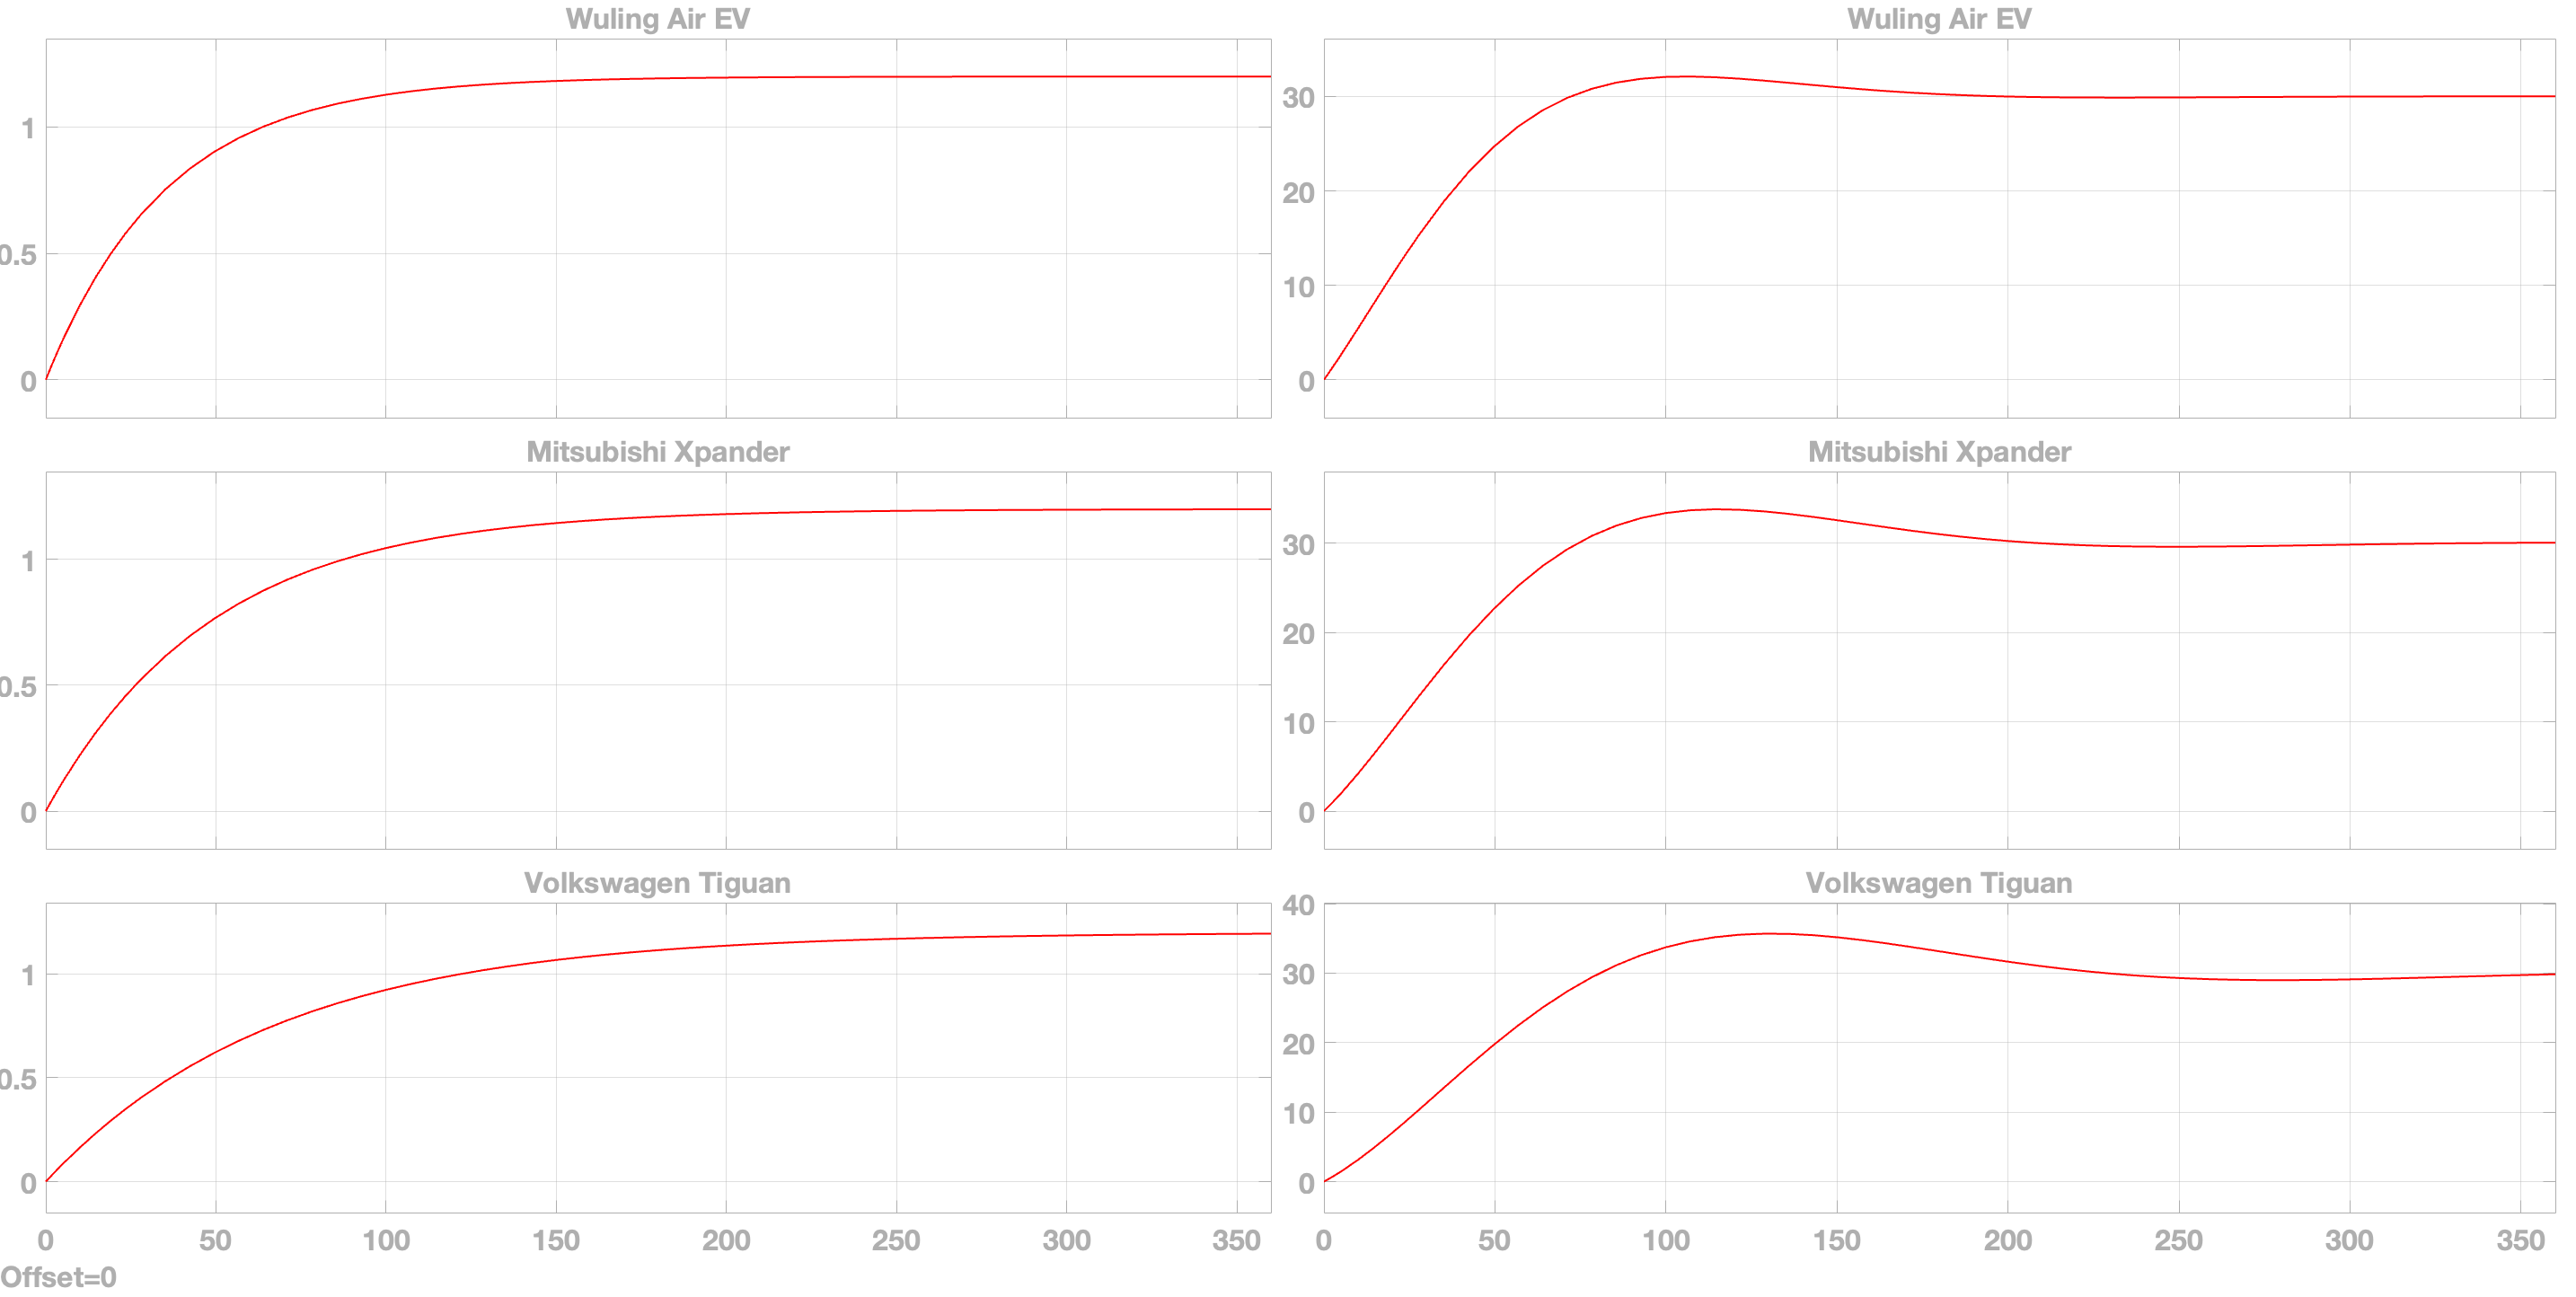
\includegraphics[width=1\linewidth]{img/15_PG.png}
    \caption{Vehicles Cruise Control System Responses (25 N*m/s \& 15 Proportional Gain)}
    \label{fig:15pg}
\end{figure}

Figure \ref{fig:15pg} shows the system response using a damping coefficient of $25 N*m / s$ and a proportional gain value of $15$. Compared to the response shown in Figure \ref{fig:25nms}, this configuration reduced the overshoot and undershoot, as well as shorter peak and settling times. Having an overshoot of $2 - 5m/s$, a rise time of $50 - 80$ seconds, a peak time of $100 - 120$ seconds, and a settling time of $200 - 250$ seconds. This outcome aligns with the expected behavior of the proportional gain, which adjusts the output proportionally to the current error. Given the improvement in settling time achieved with this value, the author proceeds to experiment with the Integral and Derivative gains to further optimize the settling time, rise time, and peak time.

\begin{figure}[htbp]
    \centering
    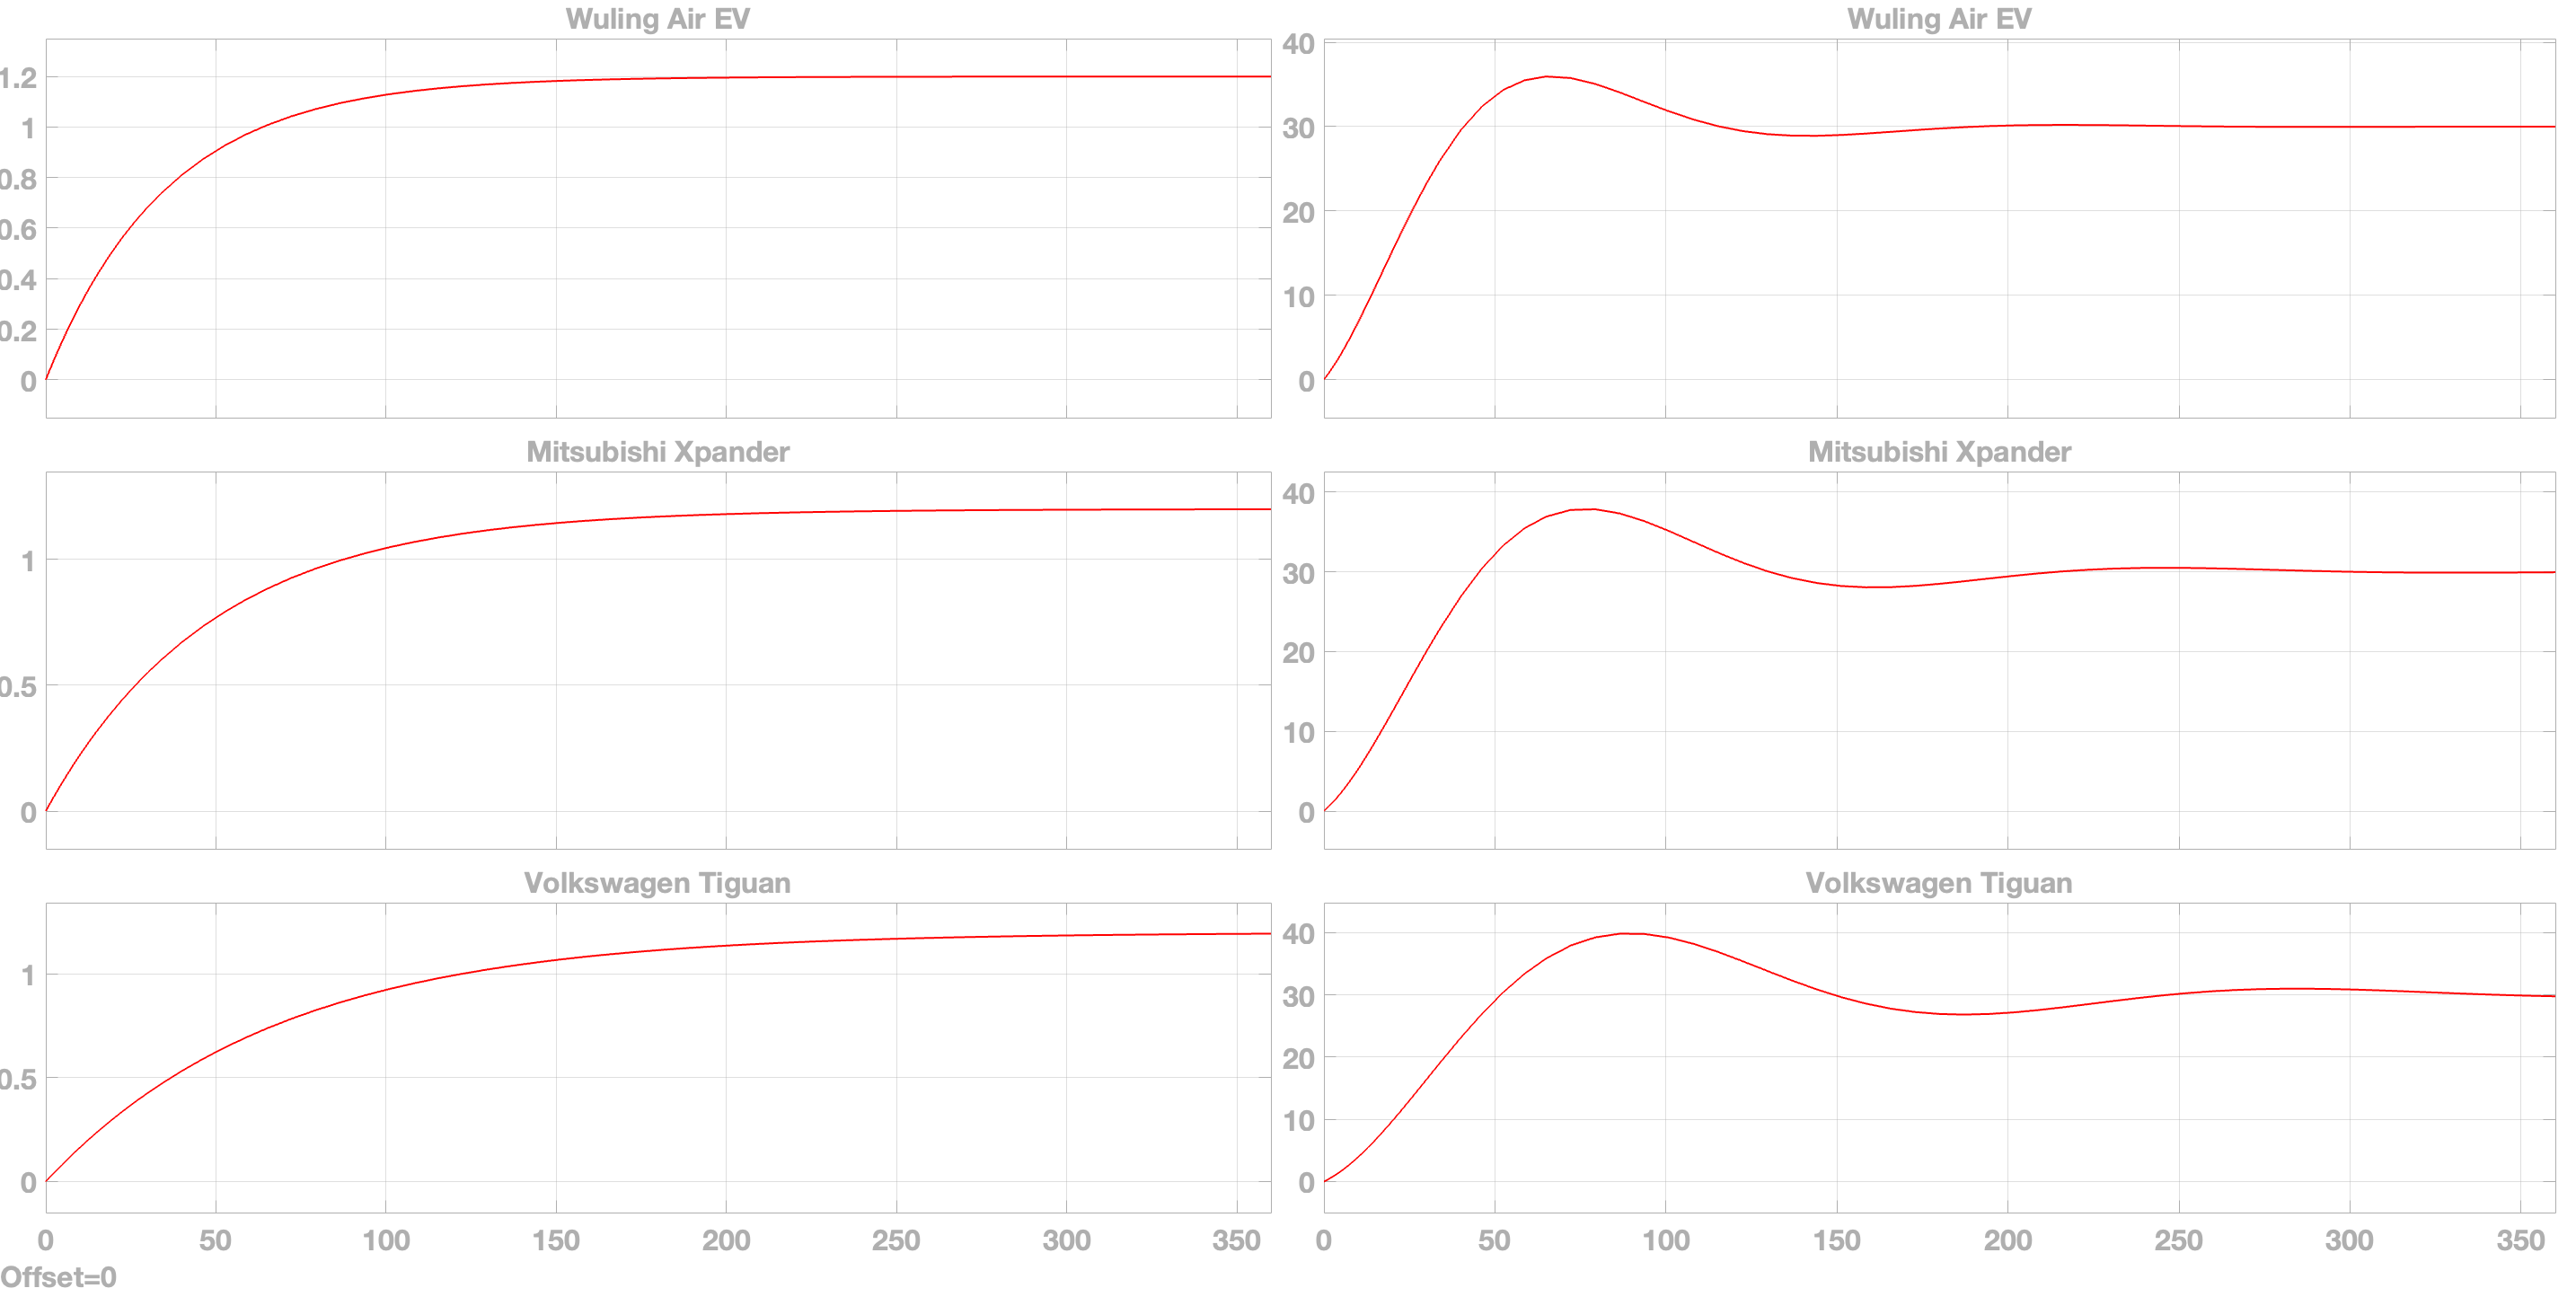
\includegraphics[width=1\linewidth]{img/15_PG_2_IG_1_DG.png}
    \caption{Vehicles Cruise Control System Responses (25 N*m/s, 15 Proportional Gain, 2 Integral Gain \& 1 Derivative Gain)}
    \label{fig:15pg2ig1dg}
\end{figure}

Figure \ref{fig:15pg2ig1dg} illustrates the system response with a damping coefficient of $25 N*m / s$, a proportional gain of $15$, an integral gain of $2$, and a derivative gain of $1$. This PID controller configuration significantly reduces the rise and peak times, albeit with increased overshoot and undershoot. Having an overshoot of $6 - 10 m/s$, an undershoot of $1 - 3 m/s$, but a rise time of $25 - 60$ seconds, and a peak time of $60 - 90$ seconds. Despite the overshoot, the higher rise time objective is achieved. This overshoot occurs because the system's response requires greater correction from the starting velocity to the desired velocity. Additionally, the author will explore how initiating the system from a non-zero velocity can enhance regulation speed and precision.

\subsubsection{Transient Response Analysis of System with Increased Starting Velocity}

\begin{figure}[htbp]
    \centering
    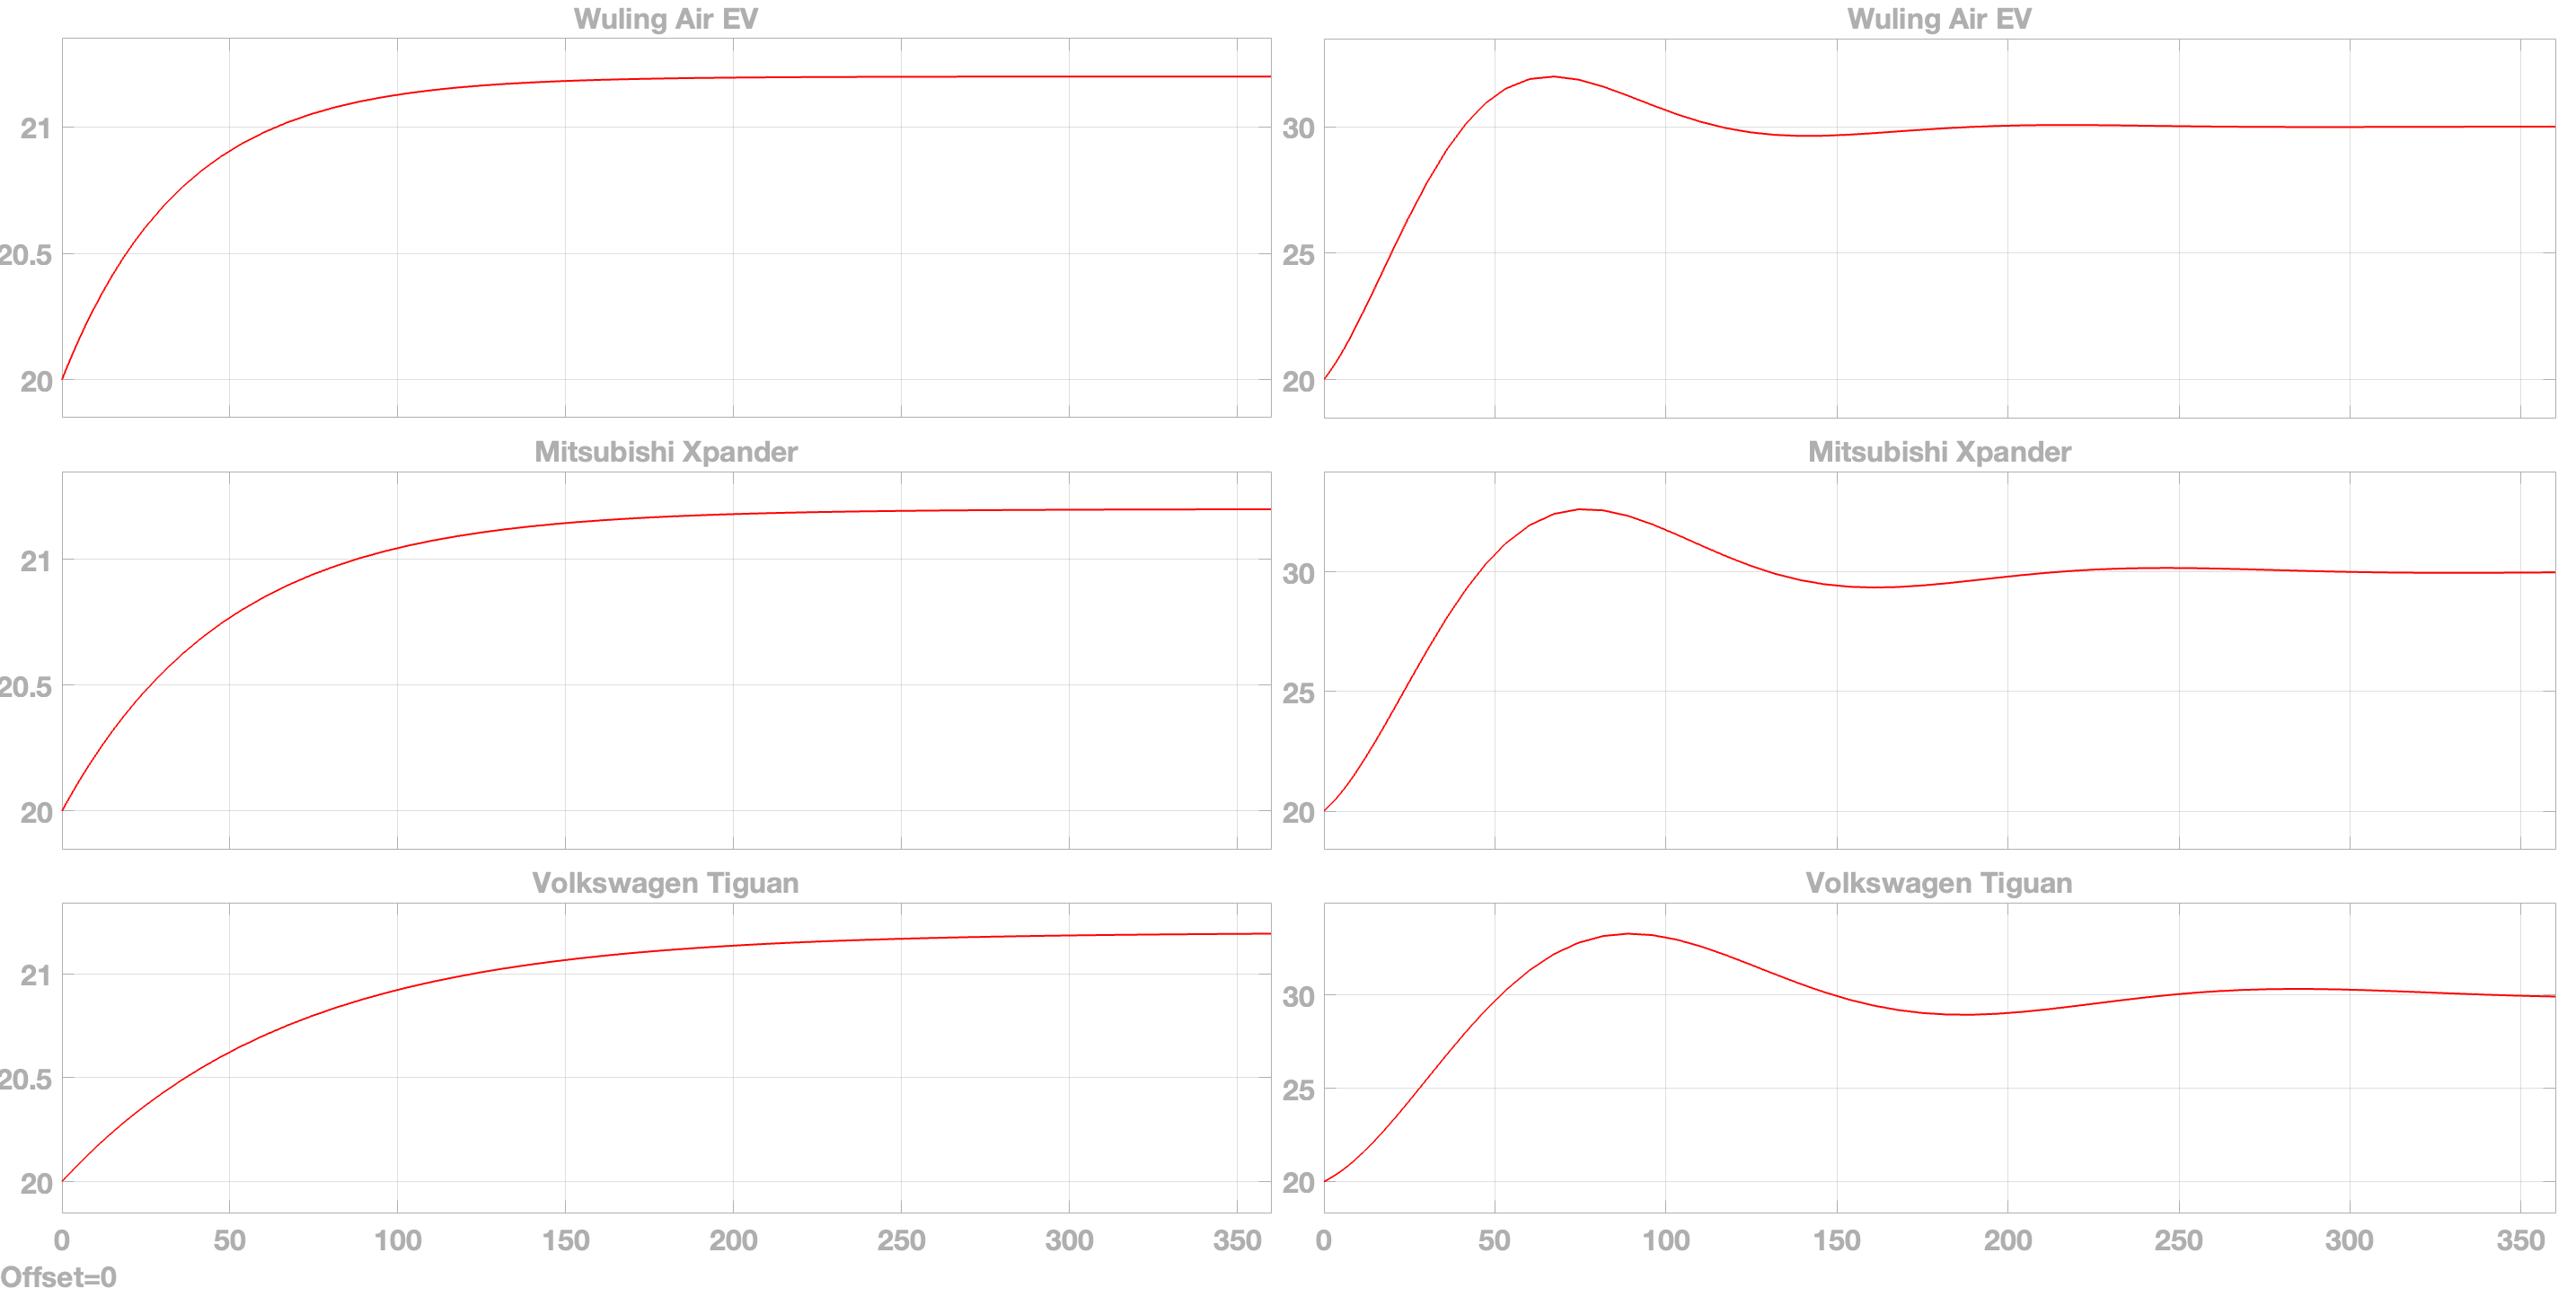
\includegraphics[width=1\linewidth]{img/20ms.png}
    \caption{Vehicles Cruise Control System Responses (25 N*m/s, 15 Proportional Gain, 2 Integral Gain \& 1 Derivative Gain) with Starting Velocity of 20m/s}
    \label{fig:20ms}
\end{figure}

Initiating the system with a starting velocity closer to the desired velocity intuitively enhances system performance, as the PID Controller requires fewer corrections and can regulate the output more precisely. In Figure \ref{fig:20ms}, the same configuration based on the setup in Figure \ref{fig:15pg2ig1dg} is depicted, but with a starting velocity of $20 m/s$. This adjustment results in significantly reduced overshoot and undershoot, typically in the range of $2 - 4 m/s$, while other aspects of the system's response remain consistent.

The author has demonstrated that system configuration significantly influences its ability to self-correct, impacting various aspects of system response including rise time, peak time, settling time, overshoot, undershoot, and steady-state error. The display of the system starting from zero velocity or any other starting velocity to the desired output demonstrates that the overshoot is proportional to the difference between them. With a clear analysis of how to engage with the system in practice, engineers can analyze the reasonable margins of overshoots and undershoots that might occur. Additionally, it is important to complete the report with a demonstration of an initial velocity that exceeds the desired velocity and its ability to correct it, shown in Figure \ref{fig:40ms}.

\begin{figure}[htbp]
    \centering
    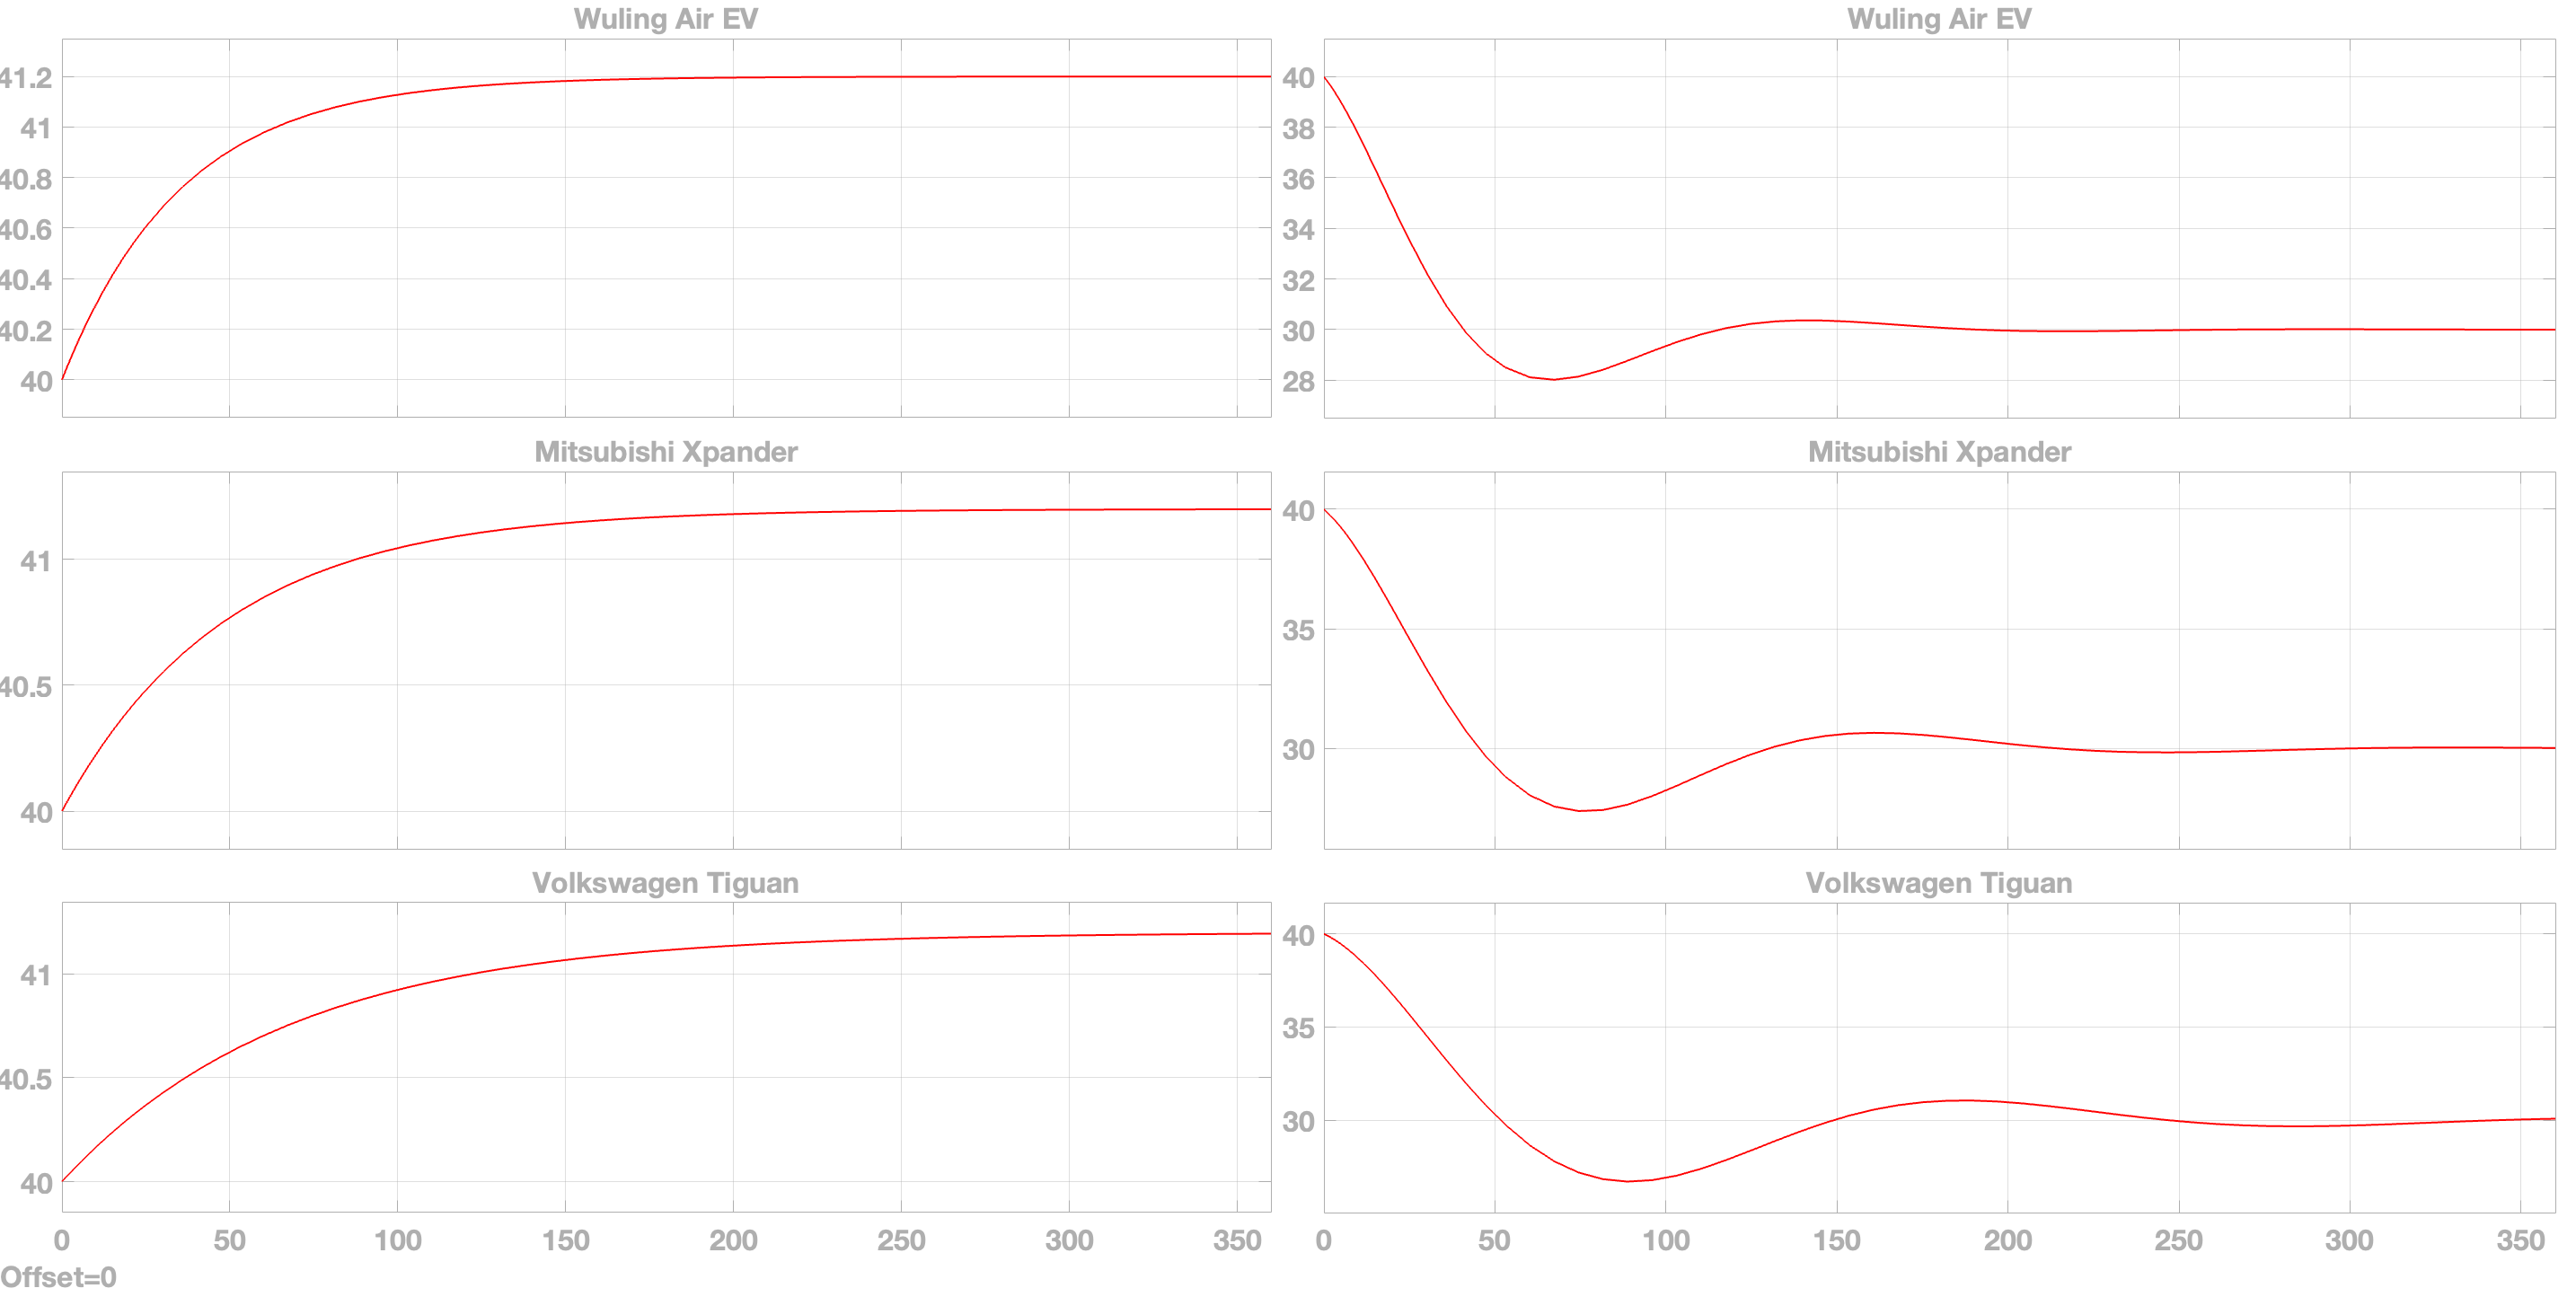
\includegraphics[width=1\linewidth]{img/40ms.png}
    \caption{Vehicles Cruise Control System Responses (25 N*m/s, 15 Proportional Gain, 2 Integral Gain \& 1 Derivative Gain) with Starting Velocity of 40ms/s}
    \label{fig:40ms}
\end{figure}

\section{Conclusion}

This report investigates a simplified version of a Vehicle Cruise Control System's dynamics, diving into modeling, simulation, control, and analysis through various experimentation procedures aimed at understanding its transient response. While different vehicle systems may vary in weight and damping coefficient, this report discusses an estimation of how the system operates, considering that the three chosen vehicles as examples may necessitate different parameters and adjustments for optimal cruise control experience in practical scenarios. Furthermore, it's important to note that this analytical approach can be scaled with different parameters, catering to the complexity of the system.

\newpage
\listoffigures
\listoftables

\newpage
\bibliographystyle{plain} % Choose a style
\bibliography{references} % Assuming your file is named 'references.bib'

\end{document}
